\documentclass{beamer}
\usepackage{beamerthemesplit}
\usepackage{graphics}
\logo{
\includegraphics[height=1cm]{psi_logo_white.png}}
\usetheme{Pittsburgh}
\usecolortheme{dove}
\beamertemplatenavigationsymbolsempty
\setbeamertemplate{footline}[frame number]
\definecolor{myback}{RGB}{175,238,238}
\setbeamercolor{structure}{bg=myback}
\usepackage[T1]{fontenc}
\newcommand{\changefont}[3] {
 \fontfamily{#1} \fontseries{#2} \fontshape{#3} \selectfont}

\title{The NeXus Data Format for muon Spectroscopy and Neutron or X-ray Scattering }
\author{Mark K\"onnecke }
\institute{Paul Scherrer Institute\\Switzerland }
\date{\today} 

\begin{document}

\begin{frame}
\titlepage
\end{frame}

\begin{frame}
\frametitle{The Predicament of the Traveling Scientist}
\begin{itemize}
\item<1->A different data format wherever she goes
\item<2->Spends lots of time converting formats or writing readers
\item<3->Waits even longer to load data from inefficient data formats
\item<4->DA requires N files in different  formats, notes, local knowledge 
\item<5->Cannot read her collaborators data
\item<6->Has to keep extra information in yet another form
\end{itemize}
\end{frame}

\begin{frame} \frametitle{NeXus Mission}
\begin{itemize}
\item Definition of a standard data format
\begin{itemize}
\item Rules
\item Validation tools
\end{itemize}
\item Promotion of NeXus
\begin{itemize}
\item Documentation
\item NeXus API
\item Outreach to the scientific community
\end{itemize}
\end{itemize}
\end{frame}


\begin{frame} \frametitle{NeXus Design}
\begin{itemize}
\item Complete data for typical use
\item Extendable, add additional data as you please
\item Self describing
\item Easy automatic plotting
\item Platform independent, public domain, efficient
\item Suitable for a wild variety of applications
\end{itemize}
\end{frame}


\begin{frame}
 \frametitle{NeXus Levels }
\begin{enumerate}
\item Physical file format and API for accessing files
\item Rules for storing data in files
\item Component and application definitions
\item NeXus Utilities
\end{enumerate}
\end{frame}


\begin{frame} \frametitle{Physical File Format }
\begin{itemize}
\item Portable, self describing, extendable, public domain
\item Hierarchical data format, NCSA, HDF-4, later HDF-5
\item HDF-5:
\begin{itemize}
\item grouping support
\item on the fly compression
\item reading/writing subsets
\item first dimension appendable
\item Public domain C, F77 access library
\item Used by: NASA, Boing, the weathermen, .... 
\end{itemize}
\item XML for those who wish to edit their data
\end{itemize}
\end{frame}


\begin{frame} \frametitle{NeXus API }
\begin{itemize}
\item NeXus-API hides complex HDF API
\item Transparent access to all three supported physical file formats
\item ANSI-C implementation
\item Bindings: C++, F77, Java, python, IDL, SWIG
\item January, 4, 2010: 1311217 files processed at PSI alone
\end{itemize}
\end{frame}

\begin{frame} \frametitle{Threads Versus NeXus}
\begin{itemize}
\item Planned: NeXus is threadsafe when each thread has its own NXhandle
\item A little work needs to be done to arrive there
\item {\color{red}BUT:} HDF-5 serialises access, no performance gain!
\item Parallel HDF5, PHDF, with a different API
\item PHDF requires: MPI, MPI-IO, parallel file system
\item A new NeXus file driver for PHDF would be required
\item Will only be implemented when the community really wants it
\end{itemize}
\end{frame}

\begin{frame} \frametitle{NeXus Objects}
\begin{itemize}
\item Files
\item Groups identified by name and a classname beginning with NX
\item Scientific data sets
\item Attributes
\item Links
\end{itemize}
\end{frame}

\begin{frame} \frametitle{Coordinate Systems}
\begin{itemize}
\item McStas Coordinate System
\item Angle based polar coordinate system
\item {\color{red}NEW: full mapping imageCIF - NeXus now possible}
\item {\color{red}NEW: General axis and transformations}
\end{itemize}
\end{frame}


\begin{frame}
\frametitle{NeXus General Rules}
\begin{itemize}
\item NeXus reserves the prefix NX for group names.  
\item Store as much as possible
\item A NeXus file has one to many NXentry groups 
\item There are two types of entries: raw data and processed data
\item Multiple different techniques in one file go into separate NXsubentries
\item If there is only one entry, the preferred name is entry, else entry1, entry2... entryn
\item If an entry or an NXsubentry conforms to an application definition, 
 the application definitions must be stated in the 
 entries definition field.
\end{itemize}
\end{frame}

\begin{frame} \frametitle{NeXus Raw Data File Structure}
\begin{tabbing}
\hspace*{1cm} \= \hspace*{1cm} \= \hspace*{1cm} \= \hspace*{1cm} \= \hspace*{1cm} \= \hspace*{1cm}\= \kill
entry:NXentry \\
 \>sample:NXsample \\
\\
 \>instrument:NXinstrument\\
 \> \> source:NXsource\\
 \> \> velocity\_selector:NXvelocity\_selector\\
 \> \> detector:NXdetector \\
 \> \> \>data[xsize,ysize], signal=1 (1)\\
 \>control:NXmonitor\\
 \> \>data\\
 \>data:NXdata\\
 \> \> link to (1)\\
\end{tabbing}
\end{frame}

\begin{frame} \frametitle{NeXus Processed Data File Structure}
\begin{tabbing}
\hspace*{1cm} \= \hspace*{1cm} \= \hspace*{1cm} \= \hspace*{1cm} \= \hspace*{1cm} \= \hspace*{1cm}\= \kill
entry:NXentry \\
 \>sample:NXsample \\
 \>processing\_name:NXprocess\\
 \> \>program \\
 \> \>version \\
 \> \>parameters:NXparameter \\
 \> \> \>raw\_file \\
 \>data:NXdata\\
 \> \> data[nx,ny,nz], signal=1\\
\end{tabbing}
\end{frame}

\begin{frame} \frametitle{{\color{red}NEW}: NXsubentry}
\begin{tabbing}
\hspace*{1cm} \= \hspace*{1cm} \= \hspace*{1cm} \= \hspace*{1cm} \= \hspace*{1cm} \= \hspace*{1cm}\= \kill
entry:NXentry \\
\>sample:NXsample\\
\>instrument:NXinstrument\\
\>.....\\
 \>{\color{red}sas:NXsubentry}\\
 \>  \>sample:NXsample \\
\\
\> \>instrument:NXinstrument\\
\> \> \> source:NXsource\\
\> \> \> velocity\_selector:NXvelocity\_selector\\
\> \> \> detector:NXdetector \\
\> \> \> \>data[xsize,ysize], signal=1 (1)\\
\> \>control:NXmonitor\\
\> \> \>data\\
\> \>data:NXdata\\
\> \> \> link to (1)\\
\end{tabbing}
\end{frame}

\begin{frame} \frametitle{{\color{red}NEW: NXcollection}}
\begin{tabbing}
\hspace*{1cm} \= \hspace*{1cm} \= \hspace*{1cm} \= \hspace*{1cm} \= \hspace*{1cm} \= \hspace*{1cm}\= \kill
\>entry,NXentry\\
\> \>measurement:NXcollection\\
\> \> \>positions:NXcollection\\
\> \> \> \>om \\
\> \> \> \>two\_theta\\
\> \> \>scalars:NXcollection\\
\> \> \> \>title\\
\> \> \> \>wavelength\\
\> \> \>data:NXdata\\
\> \> \> \>detector1\\
\> \> \> \>mca5\\
\end{tabbing}
\end{frame}

\begin{frame} \frametitle{Why the Hierarchy??}
\begin{itemize}
\item<1->Supports self description and allows short names in components
\item<2->Name, classname pair allows for multiple components of the same type
\item<3->NXentry allows for multiple datasets in the same file
\item<4->NXdata supports automatic plotting
\item<5->Take care once when writing, use n times
\end{itemize}
\end{frame}

\begin{frame}
\frametitle{Rules for Storing Data Items}
\begin{itemize}
\item Store physical values in C storage order
\item Use NeXus components and dictionary names
\item Missing names will be quickly accepted by the NIAC
\item Names: full words separated by \_
\item Specify units in same format as used by UDunits
\item Application definitions may restrict units
\end{itemize}
\end{frame}

\begin{frame}
\frametitle{{\color{red} NEW: Data Storage Exceptions}}
\begin{itemize}
\item There are situations were data has to be dumped as fast as possible in order to 
 keep up with a high data rate. Or to save disk space.
\item {\bf Data not in C storage order:} use attributes stride and offset to describe the 
 memory layout of the data.
\item {\bf Data needs scaling:}Use a NXformula group to specify a formula in muParser 
 notations plus the parameters and data necessary to do the scaling.
\item Details on both methods will be in the NeXus manual  
\end{itemize}
\end{frame}



\begin{frame} \frametitle{Associating Axis and Data, Preferred method}
\begin{tabbing}
\hspace*{1cm} \= \hspace*{1cm} \= \hspace*{1cm} \= \hspace*{1cm} \= \hspace*{1cm} \= \hspace*{1cm}\= \kill
entry:NXentry \\
 \>data:NXdata\\
 \> \> data[nx,ny,nz], signal=1, axes=x\_axis,y\_axis,z\_axis\\
 \> \> x\_axis[nx]\\
 \> \> y\_axis[ny]\\
 \> \> z\_axis[nz]\\
\end{tabbing}
\end{frame}


\begin{frame}
\frametitle{Storing Detector Data}
\begin{itemize}
\item Preserve original dimensionality of detector, if possible
\item Time-of-flight becomes last dimension
\item Highly irregular detectors:
\end{itemize}
\begin{tabbing}
\hspace*{1cm} \= \hspace*{1cm} \= \hspace*{1cm} \= \hspace*{1cm} \= \hspace*{1cm} \= \hspace*{1cm}\= \kill
entry:NXentry \\
\>instrument:NXinstrument\\
\> \>detector:NXdetector\\
\>  \> \> data[ndet], signal=1\\
\> \> \> polar\_angle[ndet], axis=1\\
\> \> \> azimuthal\_angle[ndet]\\
\> \> \> distance[ndet]\\
\end{tabbing}
\end{frame}


\begin{frame}
\frametitle{Scans}
\begin{itemize}
\item Come in all shapes and sizes
\item Captured by rules:
\begin{itemize}
\item Store all varied parameters as arrays of length NP at the appropriate place in the NeXus 
 hierarchy
\item For multi detectors, NP, number of scan points is always the first dimension
\item In NXdata: create links to counts and varied variables
\end{itemize}
\end{itemize}
\end{frame}


\begin{frame}
\frametitle{Scan Example 1: rotating sample}

\begin{tabbing}
\hspace*{1cm} \= \hspace*{1cm} \= \hspace*{1cm} \= \hspace*{1cm} \= \hspace*{1cm} \= \hspace*{1cm}\= \kill
entry:NXentry \\
 \>sample:NXsample\\
 \> \> rotation\_angle[NP], axis=1 (1) \\
 \> instrument:NXinstrument\\
 \>  \>detector:NXdetector\\
 \>  \> \>data[NP],signal=1 (2)\\
 \>control:NXmonitor\\  
 \> \>data[NP]\\  
 \>data:NXdata\\
 \> \> link to (1)\\
 \> \> link to (2) \\
\end{tabbing}
\end{frame}

\begin{frame}
\frametitle{Scan Example 2: complex scan in Q}

\begin{tabbing}
\hspace*{1cm} \= \hspace*{1cm} \= \hspace*{1cm} \= \hspace*{1cm} \= \hspace*{1cm} \= \hspace*{1cm}\= \kill
entry:NXentry \\
 \>sample:NXsample\\
 \> \> rotation\_angle[NP], axis=1 (1) \\
 \> \> phi[NP], axis=1 (2) \\
 \> \> chi[NP], axis=1 (3) \\
 \> \> h[NP], axis=1 (4), primary=1 \\
 \> \> k[NP], axis=1 (5) \\
 \> \> l[NP], axis=1 (6) \\
 \> instrument:NXinstrument\\
 \>  \>detector:NXdetector\\
 \>  \> \>data[NP],signal=1 (7)\\
 \>  \> \>polar\_angle[NP],signal=1 (8)\\
 \>data:NXdata\\
 \> \> link to (1)\\
 \> \> link to (2) \\
 \> \> link to (...) \\
 \> \> link to (8) \\
\end{tabbing}
\end{frame}


\begin{frame}
\frametitle{Scan Example 3: sample rotation, area detector}
\begin{tabbing}
\hspace*{1cm} \= \hspace*{1cm} \= \hspace*{1cm} \= \hspace*{1cm} \= \hspace*{1cm} \= \hspace*{1cm}\= \kill
entry:NXentry \\
 \>sample:NXsample\\
 \> \> rotation\_angle[NP], axis=1 (1) \\
 \> instrument:NXinstrument\\
 \>  \>detector:NXdetector\\
 \>  \> \>data[NP,xsize,ysize],signal=1 (2)\\
 \>control:NXmonitor\\  
 \> \>data[NP]\\  
 \>data:NXdata\\
 \> \> link to (1)\\
 \> \> link to (2) \\
\end{tabbing}
\end{frame}


\begin{frame}
\frametitle{Rasterisation}
\begin{itemize}
\item This is rastering a sample at different wavelengths, positions etc. 
\item Same treatment as scans, NP replaced by NR number of raster points
\item For the common case of rastering on a 2D grid one can store [nx,ny,detdim]. Be aware, though, that 
 this causes problems if the rasterisation is aborted in mid operation. 
\end{itemize}
\end{frame}


\begin{frame} \frametitle{NeXus Component and Application Definitions }
\begin{itemize}
\item Component definitions: 
 dictionaries of allowed field names for the various NeXus groups
{\changefont{cmr}{bx}{sc} 
\item Application Definitions
\begin{itemize}
\item Define what has to be in a NeXus file for a certain application
\item Defines standards
\item Another view: Contract between file producers and users about what has to be in 
 a NeXus file for a well defined purpose 
\item Validation by NXvalidate
\end{itemize}
}
\item Written in NeXus Definition Language, NXDL
\end{itemize}
\end{frame}

\begin{frame}
\frametitle{All Base Classes}
\begin{tabular}{lll}
NXaperture & NXattenuator & NXbeam\_stop \\
NXbeam     & NXbending\_magnet & NXcharacterization \\
NXcollimator & NXcrystal & NXdata \\
NXdetector   & NXdisk\_chopper & NXentry \\
NXenvironment & NXevent\_data & NXfermi\_chopper \\
NXfilter & NXflipper & NXgeometry \\
NXguide & NXinsertion\_device & NXinstrument \\
NXlog & NXmirror & NXmoderator \\
NXmonitor & NXmonochromator & NXnote \\
NXorientation & NXparameters & NXpolarizer\\
NXprocess & NXsample & NXsensor \\
NXshape & NXsource & NXtranslation\\
NXuser & NXvelocity\_selector & \\
\end{tabular}
\end{frame}


\begin{frame} \frametitle{Application Definition Process}
\begin{enumerate}
\item Construct an application definition with advice from the NIAC
\item You can also inherit from and extend an existing definition
\item Cure for a year; data should be produced in the new format in this time
\item After curation and review: this is the standard for this application type.
\end{enumerate}
\begin{itemize}
\item No promises, but the NIAC may do it for you
\begin{itemize}
\item Description of experiment
\item Minimum set of data items necessary form common use
\item Example data
\end{itemize}
\end{itemize}

\end{frame}


\begin{frame}
\frametitle{Four Steps}
\begin{enumerate}
\item {\color{blue} Think!} what ought to go into the file
\item {\color{blue}Map }this into the NeXus file structure
\item {\color{blue} Cast} this mapping into a NXDL file
\item {\color{blue} Standardize} your application definition together with the NIAC
\end{enumerate}
\end{frame}

\begin{frame}
\frametitle{Think!}
\begin{itemize}
\item What has to go into the file?
\item Minimum data necessary for common usage scenarios
\item Haggle it out with your community
\item Coverage ratio: $> 80$ \% of use cases
\end{itemize}
\end{frame}

\begin{frame}
\frametitle{Map to NeXus}
\begin{itemize}
\item Consider into which NeXus group an item might belong
\item Look in the base class for a suitable data field
\item Link the data items required for the default plot into NXdata
\end{itemize}
\end{frame}

\begin{frame}
\frametitle{From an application definition to a real NeXus file}
\begin{itemize}
\item<1->The structure defined by the application definition is the minimum
\item<2->Practical files strive to capture much more
\uncover<3->{
\item Suggested procedure:
\begin{itemize}
\item Look at each of your instruments components and the matching NeXus base class
\item Add whatever you feel like adding or the instrument scientists wants to have
\item Add whatever management wants to have (may be not in a NeXus group)
\end{itemize}
}
\item<4-> Remember: {\color{red}Adding more fields does not break application definition compliance!} 
\end{itemize}
\end{frame}

\begin{frame} \frametitle{{\color{red}NEW}: Available NeXus Application Definitions}
{\changefont{cmr}{bx}{sc} 
\begin{tabular}{lll}
NXarchive& NXmonopd & NXrefscan \\
NXreftof & NXsas & NXscan \\
NXtas & NXtofraw& NXtomo\\
NXtomophase & NXxeuler & NXxkappa\\
NXxnb & NXxrot & NXiqproc \\
NXtomoproc & NXtofsingle& NXdirectof\\
NXindirectof & NXiqproc& NXlauetof\\
NXsastof& NXsqom& NXtofraw\\
NXtofsingle& NXxas& NXxasproc\\
\end{tabular}
}
\end{frame}


\begin{frame} \frametitle{Data Format Challenges}
\begin{description}
\item<1->[Challenge 1] in science you are supposed to do new, non standard, things.  
 These of course cannot be easily cast into a standard.
\item<2->[Challenge 2] in order to establish a standard a lot of people need to agree
\item<3->[Challenge 3] a standard requires scarce scientific  programming resources for adoption 
\end{description}
\end{frame}

\begin{frame} \frametitle{Data Format Benefits}
\begin{description}
\item<1->[Benefit 1] By using a discoverable data format like NeXus, XML, HDF-5, people can at 
 least figure out  what is in the data file. 
\item<2->[Benefit 2] Using predefined names from a dictionary gives meaning to the data in a file.
\item<3->[Benefit 3] Using a shared API reduces learning costs and increases application stability.
\item<4->[Benefit 4] With NeXus, HDF-5 plus professional programming techniques a DA application can 
 read any file which contains the required data.
\item<5->[Benefit 5] Storing as much data as possible increases the likelihood that the needed 
 data is actually on file, even for unforeseen uses. 
\item<6->[Benefit 6] Application Definitions
\end{description}
\end{frame}


\begin{frame} \frametitle{Who commits to NeXus? }
\begin{figure}[!ht]
\resizebox{7cm}{5cm}{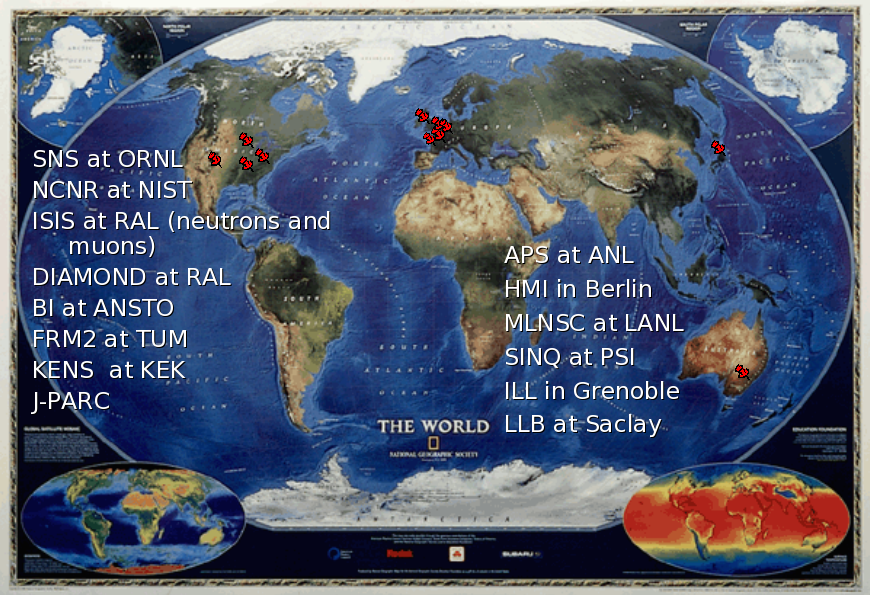
\includegraphics[width=0.75\textwidth]{nxworld.png}}\end{figure}
\end{frame}


\begin{frame} \frametitle{What You Can Do with NeXus}
\begin{enumerate}
\item Store and archive data from a wild variety of instruments
\item Store processed data
\item Store a complete workflow from raw data to publication ready data in several 
 NXentries in one file
\item Store a set of related experiments in one file
\item Define strict and validatable standards 
\end{enumerate}
\end{frame}

\begin{frame} \frametitle{NeXus Outlook}
\begin{itemize}
\item New systems tend to use NeXus
\item No competitor for a general purpose data format
\item Planned:
\begin{itemize}
\item Refine application definitions together with communities
\item Release application definitions and NXvalidate
\item Update manuals and the NeXus WWW-site
\item www.nexusformat.org, embarrasingly outdated, download manual
\end{itemize}
\end{itemize}
\end{frame}

\end{document}


\begin{frame} \frametitle{Conclusion }
\begin{itemize}
\item NeXus is a mature and capable data format
\item There is no other standard then NeXus on the horizon
\item New things are developed with NeXus everywhere, uptake at established sites is slow
\item You are invited to join the NIAC and contribute to NeXus 
\item More information: http://www.nexusformat.org (outdated, but working on it)
\end{itemize}
\end{frame}


\begin{frame} \frametitle{Example Files}
\end{frame}

\begin{frame} \frametitle{Storing Single Data Items }
\begin{itemize}\item Units have to specified
\item Locating axis, by example:
\begin{itemize}\item counts(two\_theta, time\_of\_flight), attributes: signal=1
\item two\_theta, attributes: axis=1, axis=primary 
\item time\_of\_fligth, attributes: axis=2, axis=primary
\end{itemize}\end{itemize}
\end{frame}

\begin{frame} \frametitle{NXtranslate }
\begin{itemize}\item Anything to NeXus converter:
\begin{itemize}\item Binary dump
\item FRM2
\item IPNS run
\item NeXus
\item Spec
\item XML
\end{itemize}\item Uses XML based translation file to control translation
\item Extendable via plugins
\end{itemize}
\end{frame}

\begin{frame} \frametitle{NXextract}
\begin{itemize}
\item Extracts NeXus files to binary or ASCII
\item Uses XML template file to control conversion
\item Contributed by Stephane Poirier, SOLEIL 
\end{itemize}
\end{frame}

\begin{frame} \frametitle{Another Way to use NeXus/HDF-5}
\begin{enumerate}
\item Use NXopenpath(hfil,path) to access the data in file, use introspection to 
 find out about dimensions
\item Have a dictionary mapping what you need for DA to paths
\item Keep the dictionary in a separate file
\item When you encounter a different file, just edit the dictionary file 
\end{enumerate}
\end{frame}

\begin{frame} \frametitle{McStas Coordinate System }
\begin{figure}[!ht]
\resizebox{7cm}{5cm}{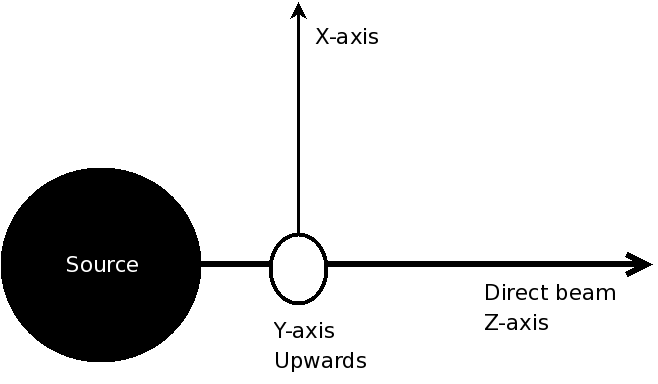
\includegraphics[width=0.75\textwidth]{mcstas.png}}\end{figure}
\end{frame}

\begin{frame} \frametitle{NeXus Simple Coordinate System }
\begin{figure}[!ht]
\resizebox{7cm}{5cm}{\includegraphics[width=0.75\textwidth]{polplane.png}}\end{figure}
\end{frame}




\begin{frame} 
\frametitle{NeXus Endorsement }
\begin{table}[!ht]
\begin{tabular}{|c|c|c|}
\hline
SNS at ORNL & SINQ at PSI\\ \hline
 NCNR at NIST & ISIS at RAL\\ \hline
 Diamond at RAL&Opal at ANSTO\\ \hline
FRM2 at TUM&KENS at KEK\\ \hline
J-Parc & IPNS at ANL\\ \hline
APS at ANL& HMI in Berlin\\ \hline
MLNSC at LANL& LLB in Saclay\\ \hline
\end{tabular}\end{table}
\end{frame}




\begin{frame} \frametitle{NeXus Levels }
\begin{enumerate}\item Physical file format
\item API for accessing files
\item Structure for organizing data in files
\item Rules for storing individual data items
\item Component and application definitions
\end{enumerate}
\end{frame}

\begin{frame} \frametitle{NXtranslate }
\begin{itemize}\item Anything to NeXus converter:
\begin{itemize}\item Binary dump
\item FRM2
\item IPNS run
\item NeXus
\item Spec
\item XML
\end{itemize}\item Uses XML based translation file to control translation
\item Extendable via plugins
\end{itemize}
\end{frame}

\begin{frame} \frametitle{NXextract}
\begin{itemize}
\item Extracts NeXus files to binary or ASCII
\item Uses XML template file to control conversion
\item Contributed by Stephane Poirier, SOLEIL 
\end{itemize}
\end{frame}


\begin{frame}[fragile] 
\frametitle{Aside: CIF Hierarchies}
CIF uses Hierarchies too, but hides them:
\uncover<1->{
\begin{semiverbatim}
\_exptl\_crystal\_description        plate\newline
\_exptl\_crystal\_colour             colourless\newline
\_exptl\_crystal\_size\_max           0.30
\end{semiverbatim}
}
\uncover<2>{
\begin{semiverbatim}
/exptl/crystal/description        plate\newline
/exptl/crystal/colour             colourless\newline
/exptl/crystal/size/max           0.30
\end{semiverbatim}
}

\end{frame}

\begin{frame}
\frametitle{Why a Common Dataformat? }

\begin{itemize}\item Today: 
\begin{itemize}\item Lots of different data formats
\item Time wasted converting data
\item Old formats no longer capable of delivering for new high throughput detectors
\item Difficult to add additional data
\item Often, for DA multiple different files needed
\item Badly documented formats
\end{itemize}\item Tomorrow, with NeXus:
\begin{itemize}
\item Single, efficient, platform independent data format
\item All information in one file
\item Self describing
\item Extendable
\end{itemize}
\end{itemize}
\end{frame}

\begin{frame} \frametitle{NeXus History }
\begin{itemize}
\item Devised from three independent proposals by Jonathan Tischler, 
  APS, Przemek Klosowski, NIST and 
 Mark Koennecke, ISIS, PSI in 94-96
\item Improved during various NOBUGS conferences
\item NeXus International Advisory Committee, NIAC, since 2003
\item Since 2003 yearly meetings of the NIAC
\item We already considered many issues!
\item Except for one year, we never had money to develop NeXus
\end{itemize}
\end{frame}


\begin{frame} \frametitle{McStas Coordinate System }
\begin{figure}[!ht]
\resizebox{7cm}{5cm}{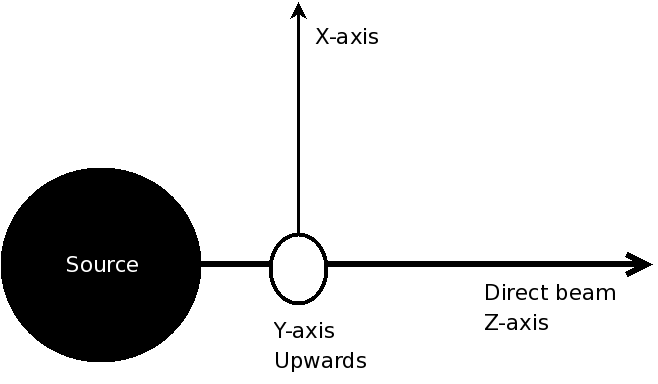
\includegraphics[width=0.95\textwidth]{mcstas.png}}\end{figure}
\end{frame}

\begin{frame} \frametitle{NeXus Simple Coordinate System }
\begin{figure}[!ht]
\resizebox{7cm}{5cm}{\includegraphics[width=0.95\textwidth]{polplane.png}}\end{figure}
\end{frame}


\begin{frame} \frametitle{Polar\_angle }
Polar angle is always relative to the previous component 
\begin{figure}[!ht]
\resizebox{7cm}{5cm}{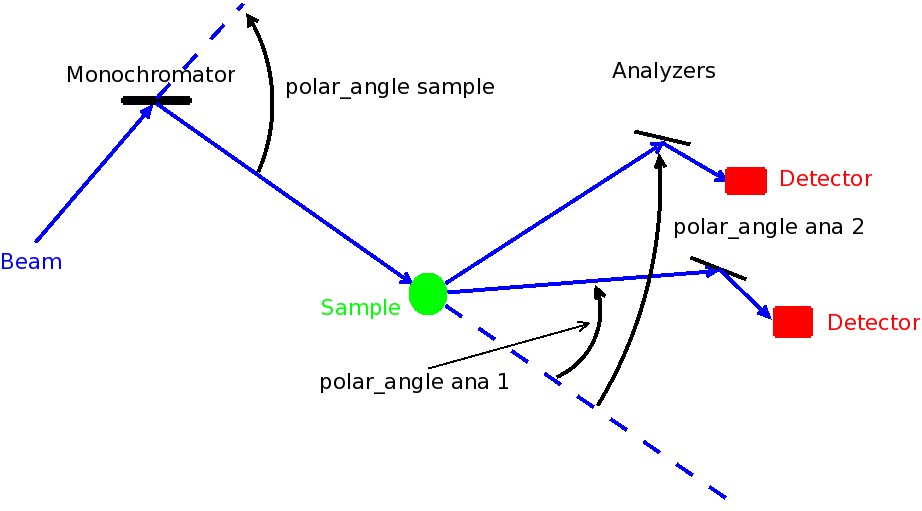
\includegraphics[width=0.95\textwidth]{polarangle.png}}\end{figure}
\end{frame}

\begin{frame} \frametitle{NXgeometry}
\begin{itemize}
\item Special group structure which can be added to any base class
\end{itemize}
\begin{tabbing}
\hspace*{1cm} \= \hspace*{1cm} \= \hspace*{1cm} \= \hspace*{1cm} \= \hspace*{1cm} \= \hspace*{1cm}\= \kill
geometry:NXgeometry \\
 \>translation:NXtranslation \\
\> \>translation[3]\\
\>shape:NXshape\\
\> \>shape: nxbox|nxcylinder|nxsphere\\
\> \>size[]\\
\>orientation:NXorientation\\
\> \>vector[3]\\
\end{tabbing}
\end{frame}


\begin{frame} \frametitle{{\color{red}NEW: NeXus Transformations}}
\begin{itemize}
\item Learning from imageCIF: be precise enough in axis descriptions to construct transformation 
 matrices 
\item Allows to calculate absolute positions of components in the laboratory coordinate systems
\item Can directly convert from a detector coordinate system to  
 vectors in Lab coordinate system
\item Calculate things like impact of primary beam on detector, SAS
\item Allows arbitray axis to be expressed
\item Intuitively describe an instrument with angles and translations and still be able
 to recover absolute coordinates
\item Attributes: transformation\_type, vector added 
\item Expressing dependency still to be resolved
\item Full mapping between imageCIF and NeXus now possible
\end{itemize}
\end{frame}


\begin{frame} \frametitle{Transformation Matrices}
\begin{math}
T = \left( \begin{array}{cccc}
1 & 0 & 0 & x\\
0 & 1 & 0 & y\\
0 & 0 & 1 & z\\
0 & 0 & 0 & 1\\
\end{array} \right)
\end{math}

\begin{math}
\onslide+<2-> 
R = \left( \begin{array}{cccc}
r11 & r12 & r13 & 0\\
r21 & r22 & r23 & 0\\
r31 & r32 & r33 & 0\\
0 & 0 & 0 & 1\\
\end{array} \right)
\end{math}

\end{frame}

\begin{frame} \frametitle{Combining Transformations}
\begin{figure}[!ht]
\resizebox{7cm}{5cm}{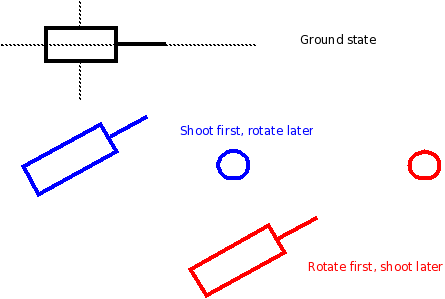
\includegraphics[width=0.75\textwidth]{rotcombi.png}}\end{figure}
\end{frame}

\begin{frame} \frametitle{Some Properties}
\begin{itemize}
\item Transformations can be combined by matrix multiplications
\item Individual matrices can be derived by looking at the situation when everything else is 0
\item Absolute positions can be obtained by multiplying the resulting matrix with its transpose
\item Defines new coordinate systems at components
\end{itemize}
\end{frame}



\begin{frame} \frametitle{Information Required}
\begin{description}
\item[type] rotation or translation
\item[direction] vector around which rotated or translated
\item[value] The angle of rotation or the length of translation
\item[dependency] The order of operations to place a component
\end{description}
\end{frame}


\begin{frame} \frametitle{NeXus Axis Mapped}
\begin{itemize}
\item rotation\_angle, polar\_angle, rotate 0 1 0
\item azimuthal\_angle, rotate 0 0 1
\item distance, translate 0 0  1
\item chi, rotate 0 0 1
\item phi rotate, 0 1 0
\item NeXus polar coordinate system: rotate azimuthal\_angle, rotate polar\_angle, 
 translate by distance
\end{itemize}
\end{frame}

\begin{frame} \frametitle{NeXus Implementation}
\begin{itemize}
\item Polar coordinate system: implied
\item General axis: attributes transformation\_type, vector
\item Axis dependency: description will be defined very soon
\end{itemize}
\end{frame}

\begin{frame} \frametitle{Associating Axis and Data}
\begin{itemize}
\item Data and axis live in the same NXgroup
\end{itemize}
\begin{tabbing}
\hspace*{1cm} \= \hspace*{1cm} \= \hspace*{1cm} \= \hspace*{1cm} \= \hspace*{1cm} \= \hspace*{1cm}\= \kill
entry:NXentry \\
 \>data:NXdata\\
 \> \> data[nx,ny,nz], signal=1\\
 \> \> x\_axis[nx], axis=1\\
 \> \> y\_axis[ny], axis=2\\
 \> \> z\_axis[nz], axis=3\\
\end{tabbing}
\end{frame}

\begin{frame} \frametitle{Multiple Axis}
\begin{tabbing}
\hspace*{1cm} \= \hspace*{1cm} \= \hspace*{1cm} \= \hspace*{1cm} \= \hspace*{1cm} \= \hspace*{1cm}\= \kill
entry:NXentry \\
 \>data:NXdata\\
 \> \> data[nx,ny,nz], signal=1\\
 \> \> x\_axis[nx], axis=1, primary=1\\
 \> \> alternate\_x\_axis[nx], axis=1\\
 \> \> y\_axis[ny], axis=2\\
 \> \> z\_axis[nz], axis=3\\
\end{tabbing}
\end{frame}




\begin{frame} \frametitle{Example: WONI}
\begin{figure}[!ht]
\resizebox{7cm}{5cm}{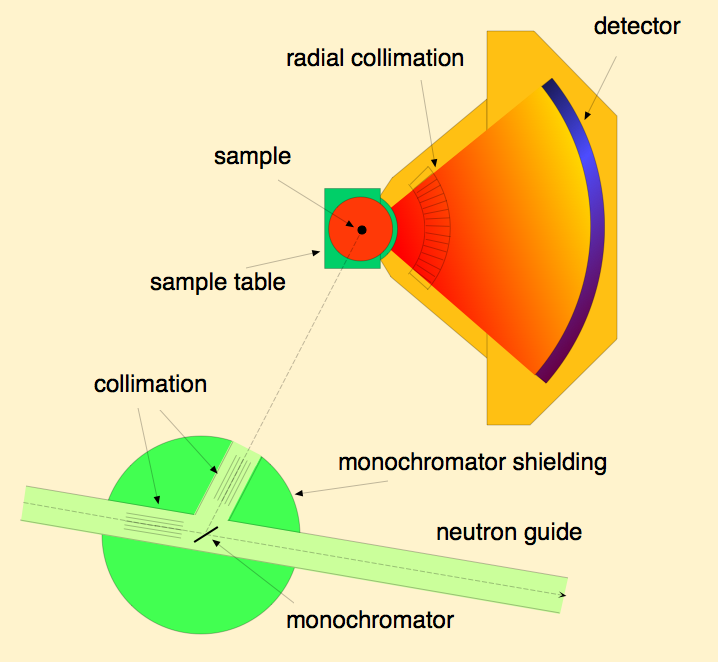
\includegraphics[width=0.85\textwidth]{dmc.png}}\end{figure}
\end{frame}

\begin{frame} \frametitle{WONI Plot}
\begin{figure}[!ht]
\resizebox{7cm}{5cm}{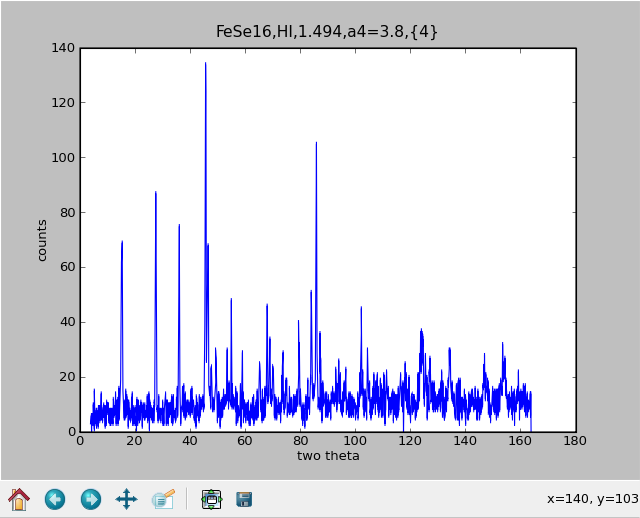
\includegraphics[width=0.85\textwidth]{powderimage.png}}\end{figure}
\end{frame}


\begin{frame}
\frametitle{Think! for WONI}
\begin{itemize}
\item Common usage is Rietveld analysis or profile analysis
\item Data required:
\begin{itemize}
\item Title
\item Sample name
\item Wavelength
\item Counts versus two\_theta
\item Monitor, for normalisation
\end{itemize}
\end{itemize}
\end{frame}


\begin{frame} \frametitle{Mappings for WONI}
\begin{tabbing}
\hspace*{1cm} \= \hspace*{1cm} \= \hspace*{1cm} \= \hspace*{1cm} \= \kill
\uncover<1-> {
entry:NXentry \\
\>title\\
\>definition\\
}
\uncover<2->{
 \>sample:NXsample \\
 \> \> name \\
}
\uncover<3->{
 \>instrument:NXinstrument\\
 \> \>monochromator:NXmonochromator\\
 \> \> \>wavelength\\
}
\uncover<4->{
 \> \> detector:NXdetector \\
 \> \> \>data[ndet], signal=1 (1)\\
 \> \> \>polar\_angle[ndet], axis=1 (2)\\
}
\uncover<5->{
\>control:NXmonitor\\
\> \>data\\
}
\uncover<6-> {
\>data:NXdata\\
\> \>link to (1)\\
\> \>link to (2)\\
}
 \end{tabbing}
\end{frame}


\begin{frame} \frametitle{What about ONOKI?}
\begin{itemize}
\item<1->ONOKI: ONe Of a Kind Instrument
\item<2->{\color{blue}Think!} what you want to store
\item<3->{\color{blue}Map} the list into the appropriate NeXus base classes. It helps to 
 look at each of the components ONOKI is assembled from and to decide what you wish 
 to store for each of them. 
\item<4->The next one to copy ONOKI is well advised to copy what you did NeXus file wise, 
 otherwise she will not be able to reuse your software!
\end{itemize}
\end{frame}
